\documentclass[10pt,a4paper]{article}
\usepackage[T1]{fontenc}
\usepackage[utf8]{inputenc}
\usepackage{lmodern,microtype}
\usepackage[a4paper,margin=22mm,headheight=14pt]{geometry}
\usepackage{amsmath,amssymb,bm}
\usepackage{booktabs,longtable,array,tabularx}
\usepackage{enumitem,xcolor,graphicx}
\usepackage{tikz}
\usetikzlibrary{arrows.meta,positioning}
\usepackage{listings,fancyhdr,hyperref,bookmark,float,lastpage,titlesec}
\definecolor{uwblue}{RGB}{20,55,105}
\definecolor{softblue}{RGB}{235,242,250}
\definecolor{codegray}{RGB}{248,248,248}
\hypersetup{colorlinks=true,linkcolor=uwblue,urlcolor=uwblue,
 pdftitle={Deconvolution GUI: Program Description and Numerical Methods},
 pdfauthor={},pdfsubject={Documentation of the dekonwolucje software},
 pdfkeywords={deconvolution, PSF, Wiener, Richardson-Lucy, blind deconvolution, PyTorch, CUDA}}
\pagestyle{fancy}\fancyhf{}\lhead{Deconvolution GUI}\rhead{Version 0.103.2}\cfoot{\thepage\ / \pageref{LastPage}}
\titleformat{\section}{\Large\bfseries\color{uwblue}}{\thesection}{0.7em}{}
\titleformat{\subsection}{\large\bfseries\color{uwblue}}{\thesubsection}{0.7em}{}
\setlist{nosep,leftmargin=1.6em}\setlength{\parindent}{0pt}\setlength{\parskip}{5pt}\renewcommand{\arraystretch}{1.18}
\lstset{basicstyle=\ttfamily\small,backgroundcolor=\color{codegray},frame=single,rulecolor=\color{black!15},breaklines=true,columns=fullflexible,showstringspaces=false}
\newcommand{\code}[1]{\texttt{#1}}
\newcommand{\calF}{\mathcal{F}}
\newcommand{\norm}[1]{\left\lVert #1\right\rVert}
\newcommand{\boxnote}[1]{\begin{center}\fcolorbox{uwblue!55}{softblue}{\begin{minipage}{0.92\linewidth}#1\end{minipage}}\end{center}}
\begin{document}
\begin{titlepage}\thispagestyle{empty}\centering
\vspace*{18mm}{\Huge\bfseries\color{uwblue} Deconvolution GUI\par}\vspace{4mm}
{\LARGE Program Description and Numerical Methods\par}\vspace{13mm}{\Large Version 0.103.2\par}
\vfill\vspace{8mm}{\large \url{https://github.com/rkotynski/dekonwolucje}\par}\vfill
\begin{minipage}{0.86\textwidth}\small
This document describes the graphical workflow, numerical data model, convolution operators, implemented deconvolution methods, quality criteria, automatic parameter tuning, and software architecture of the \code{dekonwolucje} project. The software is distributed under the MIT License. Source-code comments and internal identifiers remain in English independently of the selected English or Polish GUI language.
\end{minipage}\vspace{12mm}{\large August 2026\par}
\end{titlepage}
\pagenumbering{arabic}\tableofcontents\clearpage

\section{Purpose and scope}
The program is a desktop research application for restoration of grayscale images blurred by a point-spread function (PSF) and contaminated by noise. It supports non-blind deconvolution with a supplied PSF and blind deconvolution in which both the latent image and the PSF are updated. The GUI separates source-data preparation, committed PSF selection, algorithm parameters, and result assessment.

The same committed calculation image and calculation PSF are used by all algorithms, synthetic degradation, reblur metrics, and blind-PSF initialization. NumPy/SciPy methods and PyTorch variants are available. PyTorch uses \code{float32} by default and can use CUDA when requested and available.

\subsection{AI-assisted development disclosure}
Parts of the software and documentation were prepared with assistance from tools based on large language models (LLMs). Their suggestions were incorporated as part of the development process. This assistance does not replace independent verification: numerical methods, implementation details, parameter choices, and reconstructed results should be validated for the intended scientific application.

\section{Forward model and boundary conditions}
Let $f$ be the unknown image, $h$ the PSF, $g$ the measured image, and $n$ additive noise. The discrete model is
\begin{equation}g=\mathcal{H}f+n.\end{equation}
The project deliberately distinguishes two operators.

\subsection{Zero-boundary linear convolution}
Most iterative methods and synthetic degradation use linear convolution with zero values outside the image, followed by the exact centered \emph{same} crop. The full FFT canvas has size
\begin{equation}(M+M_h-1)\times(N+N_h-1).\end{equation}
The corresponding adjoint $\mathcal{H}_{\rm lin}^{*}$ is the transpose of this exact cropped operator, including the asymmetric convention needed for even kernels.

\subsection{Circular FFT model}
The closed-form Wiener inverse uses circular convolution because the operator is diagonal in the discrete Fourier basis. With
\begin{equation}G=\calF\{g\},\qquad H=\calF\{h_0\},\end{equation}
where the centered PSF is embedded on the image grid and shifted to the FFT origin,
\begin{equation}\mathcal{H}_{\rm circ}f=\operatorname{Re}\left\{\calF^{-1}[H\calF\{f\}]\right\}.\end{equation}
\boxnote{Linear and circular boundary models are not identical. A Wiener result can differ near the borders from an iterative result even when both use the same numerical PSF.}

\section{Committed calculation image and PSF}
\subsection{Source arrays and reset}
The program retains the image and PSF loaded from disk or generated in the GUI as source arrays. \textbf{Reset thresholds / PSF selection} restores these sources. In parallel it stores one committed pair: the thresholded calculation image and the thresholded, cropped, nonnegative, unit-sum calculation PSF.

\subsection{Image and PSF floors}
For nonnegative data $x$ with maximum $m$ and floor $T$, the applied mapping is
\begin{equation}
x_T=\begin{cases}0,&x\leq T,\\[1mm]m\dfrac{x-T}{m-T},&x>T,\end{cases}
\end{equation}
for $0<T<m$. Thus the background is removed and the surviving range is stretched to the original maximum. The PSF floor is specified as a fraction $q$ of the source PSF peak, $T_p=q p_{\max}$.

\subsection{Rectangular PSF selection and normalization}
After thresholding, all full-array samples outside the accepted red rectangle are set to zero. A compact kernel of height $M_h$ and width $N_h$ is extracted around the selected center. Missing samples are zero-padded when the rectangle extends beyond the source array. The calculation PSF is
\begin{equation}
h[u,v]\leftarrow\frac{\max(h_{\rm crop}[u,v],0)}{\sum_{u,v}\max(h_{\rm crop}[u,v],0)},
\end{equation}
so that $h\geq0$ and $\sum h=1$.

Pending slider and rectangle changes do not alter the histogram or calculation data until \textbf{Apply thresholds / PSF selection now} is pressed. The rectangle can be moved, resized by edges or corners, or scaled about its center with the mouse wheel.

\subsection{Automatic initial support}
The initial support suggestion estimates the border median $b$ and a robust noise scale
\begin{equation}\sigma_b\approx1.4826\,\operatorname{median}(|p_{\partial}-b|).\end{equation}
Pixels are active when
\begin{equation}p[u,v]>\max\left(b+3\sigma_b,10^{-2}p_{\max}\right).\end{equation}
Width and height are estimated independently, which is useful for motion blur or astigmatic PSFs. The proposal remains editable.

\section{Graphical workflow}
\subsection{Tab 1: image and PSF}
The main actions are ordered as: \textbf{Load image}, \textbf{Load PSF}, \textbf{Generate test image}, \textbf{Generate selected PSF}, and \textbf{Generate degraded input}. Previews, histograms, and resolution labels describe the committed calculation data. If source image and PSF arrays have different dimensions, the smaller array is centered on a common zero-padded canvas; no resampling is performed by this synchronization.

\subsection{Tab 2: thresholds and calculation PSF}
Two 256-bin histograms are located above the corresponding threshold controls. In full-array PSF preview, the area outside the committed rectangle is black because it is numerically zero. The compact preview shows the cropped, normalized kernel.

\textbf{Optimize PSF floor + Wiener K} searches for a plausible PSF floor and Wiener regularization. With a reference image it minimizes reconstruction MSE. Without a reference, the floor is constrained by robust PSF-background statistics and GCV selects $K$ conditionally for each fixed PSF candidate. Kernels that collapse to a few samples or lose nearly all mass are rejected or penalized.

\subsection{Tab 3: algorithm}
Tab 3 selects the reconstruction method and parameters. Optional Wiener initialization, TV processing, and neural denoising are explicit. Auto tuning freezes their enabled/disabled state at the start, so parameters of disabled stages are not changed. Blind algorithms take the PSF width and height directly from the rectangle in Tab 2.

\subsection{Tab 4: results}
All stored iterations are assessed in batches, using Torch/CUDA where practical. After reconstruction the best iteration is selected and \textbf{Auto levels} is applied. Black and white controls span the full normalized display interval, maintain a positive gap, and alter visualization only. Cached histograms provide approximate percentiles without repeated full-image sorting.

\section{Wiener filtering}
Every Wiener stage uses explicit FFT and inverse FFT operations. For scalar $K$ and optional normalized noise spectrum $N[k,l]$,
\begin{equation}
\widehat F[k,l]=\frac{H^*[k,l]G[k,l]}{|H[k,l]|^2+K N[k,l]},
\end{equation}
followed by
\begin{equation}\widehat f=\operatorname{Re}\{\calF^{-1}[\widehat F]\}.\end{equation}
The obsolete magnitude-of-IFFT output was removed because it is nonlinear and converts negative ringing into positive intensity.

For fixed PSF, generalized cross-validation uses the leverage
\begin{equation}L_H=\frac{|H|^2}{|H|^2+KN},\qquad R_H=1-L_H,
\end{equation}
and a normalized cost of the form
\begin{equation}
\operatorname{GCV}(K)=\frac{\langle|R_HG_c|^2\rangle/\langle|G_c|^2\rangle}{\langle R_H\rangle^2},
\end{equation}
where $G_c$ is the spectrum of the mean-centered measured image. GCV selects $K$ for a fixed PSF; it is not used as unrestricted proof that a strongly thresholded PSF is physically correct.

\section{Richardson--Lucy family}
\subsection{Classical Richardson--Lucy}
The multiplicative update is
\begin{equation}
f^{(t+1)}=f^{(t)}\odot\mathcal{H}_{\rm lin}^{*}\left[\frac{g}{\mathcal{H}_{\rm lin}f^{(t)}+\varepsilon}\right].
\end{equation}
The implementation uses the exact adjoint of the zero-boundary linear \emph{same} operator. Initialization can be a constant image or a Wiener result. Nonnegativity, TV processing, and a neural denoiser can be applied.

\subsection{Richardson--Lucy--Wiener}
This experimental hybrid performs an RL update and then a Wiener operation in every iteration. It combines multiplicative data correction with frequency-domain regularization controlled by $K$.

\subsection{Richardson--Lucy--Rosen}
The Rosen variant replaces ordinary back-projection by nonlinear spectral correlation
\begin{equation}
C_{L,M}=(|F_1|+\varepsilon)^L(|F_2|+\varepsilon)^M
\exp[i(\arg F_1-\arg F_2)].
\end{equation}
Smaller exponents emphasize phase. An optional relaxation moves $L$ and $M$ toward one during the iteration.

\section{Landweber, Kaczmarz, and Adam methods}
\subsection{Landweber}
The classical update is gradient descent on the least-squares data term:
\begin{equation}
f^{(t+1)}=f^{(t)}+\alpha\mathcal{H}_{\rm lin}^{*}(g-\mathcal{H}_{\rm lin}f^{(t)}).
\end{equation}
The Wiener-preconditioned version transforms the adjoint residual $d$ as
\begin{equation}
\widetilde d=\operatorname{Re}\left\{\calF^{-1}\left[\frac{\calF\{d\}}{|H|^2+KN}\right]\right\}
\end{equation}
and applies $f^{(t+1)}=f^{(t)}+\alpha\widetilde d$.

\subsection{Block Kaczmarz}
The block Kaczmarz implementation is an experimental ART-style method. Rectangular observation blocks are visited, local residuals are back-projected, and relaxed corrections are applied to the corresponding reconstruction regions. It avoids explicit construction of the very large convolution matrix.

\subsection{PyTorch Adam TV-MAP}
The non-blind Adam method minimizes
\begin{equation}J(f)=\frac12\norm{\mathcal{H}_{\rm lin}f-g}_2^2+\lambda_f\operatorname{TV}(f)
\end{equation}
with automatic differentiation. Candidate parameter sets can be processed in batches. Nonnegativity is enforced by projection when selected.

\section{Blind deconvolution}
\subsection{Blind Richardson--Lucy}
Blind RL alternates the image update with a PSF update obtained from correlation of the current image estimate and the relative-blur ratio. The PSF is cropped to the Tab-2 dimensions, projected to nonnegative values, and normalized after each update. Initialization can use the current calculation PSF or a rectangular Gaussian. Optional rotational projection imposes symmetry.

\subsection{Blind Adam TV-MAP}
The blind PyTorch method jointly minimizes
\begin{equation}
J(f,h)=\frac12\norm{h*f-g}_2^2+\lambda_f\operatorname{TV}(f)+\lambda_h\operatorname{TV}(h).
\end{equation}
After every Adam step the PSF is projected onto $h\geq0$ and $\sum h=1$, with optional rotational symmetry. Separate learning rates are used for image and PSF.

\boxnote{Blind deconvolution is intrinsically non-unique. PSF width, image sharpness, noise, regularization, initialization, and stopping iteration can compensate for one another.}

\section{Metrics and best-iteration selection}
With an independent reference, the program evaluates MSE, PSNR, and SSIM. For normalized peak value one,
\begin{equation}\operatorname{PSNR}=10\log_{10}(1/\operatorname{MSE}).\end{equation}
Without a reference it uses a composite no-reference criterion including reblur consistency, intensity preservation, total variation, and residual whiteness. For candidate $\widehat f$ the residual is
\begin{equation}r=\mathcal{H}_{\rm lin}\widehat f-g.\end{equation}
Residual whiteness is estimated from short-range normalized autocorrelations of $r-\bar r$. Metrics for the history are computed in batches and cached, so returning to the best iteration does not rerun postprocessing.

\section{Auto tuning and cancellation}
Auto evaluates parameter candidates, using batched implementations when possible. Parameters belonging to optional stages that were disabled when tuning started are frozen. Auto calculations run in an isolated numerical process. \textbf{Cancel Auto} first requests cooperative stopping; if the current numerical iteration does not return within five seconds, the worker process is terminated while the Qt GUI process remains alive.

\section{Batch processing and CUDA}
PyTorch variants operate on stacks of candidates where possible. The key choices are: default \code{float32}; cached spectra for fixed PSFs; differentiable FFT convolution for changing PSFs; memory-limited chunking; grouping of blind-history frames by PSF shape; and CPU fallback when CUDA is unavailable or memory allocation fails. GPU acceleration is most useful for large images, many iterations, and candidate batches.

\section{Software architecture}
\begin{figure}[H]\centering
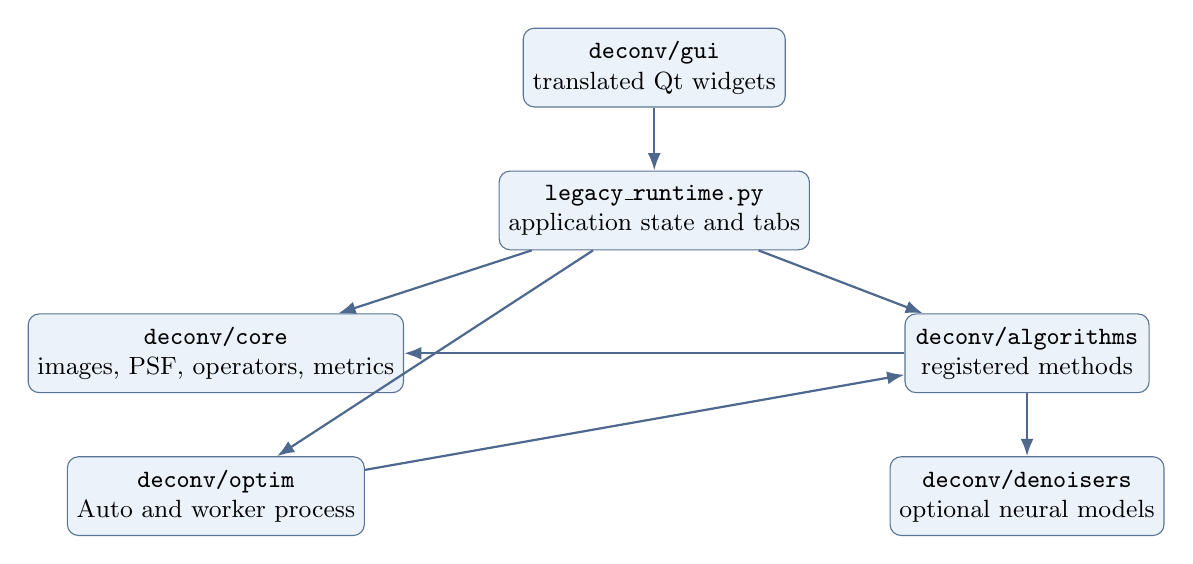
\begin{tikzpicture}[node distance=8mm and 12mm,box/.style={draw=uwblue!70,rounded corners,fill=softblue,align=center,minimum width=31mm,minimum height=10mm,font=\small},arr/.style={-{Latex[length=2.2mm]},thick,draw=uwblue!75}]
\node[box] (gui) {\code{deconv/gui}\\translated Qt widgets};
\node[box,below=of gui] (legacy) {\code{legacy\_runtime.py}\\application state and tabs};
\node[box,below left=of legacy] (core) {\code{deconv/core}\\images, PSF, operators, metrics};
\node[box,below right=of legacy] (alg) {\code{deconv/algorithms}\\registered methods};
\node[box,below=of core] (optim) {\code{deconv/optim}\\Auto and worker process};
\node[box,below=of alg] (den) {\code{deconv/denoisers}\\optional neural models};
\draw[arr](gui)--(legacy);\draw[arr](legacy)--(core);\draw[arr](legacy)--(alg);\draw[arr](legacy)--(optim);\draw[arr](alg)--(core);\draw[arr](alg)--(den);\draw[arr](optim)--(alg);
\end{tikzpicture}\caption{Main project modules and dependencies.}\end{figure}

The GUI supports exactly English and Polish. English source strings are stable identifiers. Translated widget wrappers preserve canonical English algorithm names and configuration values. The selected language is stored in the active JSON profile; source comments, docstrings, and numerical identifiers remain English.

The default settings profile is stored in the user configuration directory. On Linux this is normally \code{\textasciitilde/.config/dekonwolucje}, unless \code{XDG\_CONFIG\_HOME} is set. The last profile and image directory are remembered.

\section{Algorithm registry}
\begin{longtable}{>{\raggedright\arraybackslash}p{0.31\textwidth}>{\raggedright\arraybackslash}p{0.61\textwidth}}
\toprule\textbf{GUI identifier}&\textbf{Role}\\\midrule\endfirsthead
\toprule\textbf{GUI identifier}&\textbf{Role}\\\midrule\endhead
Wiener&Closed-form circular FFT/IFFT inverse.\\
Richardson-Lucy&Multiplicative RL with exact linear-same adjoint.\\
Richardson-Lucy-Wiener&RL followed by Wiener filtering each iteration.\\
Richardson-Lucy-Rosen&RL-like nonlinear spectral-correlation variant.\\
Blind Richardson-Lucy&Alternating image and PSF updates.\\
Landweber&Least-squares gradient descent.\\
Landweber Wiener-preconditioned&Landweber with spectral gradient preconditioning.\\
Block Kaczmarz&Experimental block/ART residual projections.\\
Torch batch Wiener&Batched PyTorch/CUDA Wiener inverse.\\
Torch batch Richardson-Lucy&Batched RL.\\
Torch batch Richardson-Lucy-Wiener&Batched hybrid RL/Wiener.\\
Torch batch Richardson-Lucy-Rosen&Batched Rosen variant.\\
Torch batch Landweber&Batched Landweber.\\
PyTorch Adam TV-MAP&Non-blind differentiable MAP optimization.\\
PyTorch Blind Adam TV-MAP&Joint image/PSF MAP optimization.\\\bottomrule
\end{longtable}

\section{Installation, testing, and extension}
\begin{lstlisting}[language=bash]
python -m venv .venv
source .venv/bin/activate
python -m pip install --upgrade pip
python -m pip install -e .
dekonwolucje
\end{lstlisting}
Alternative launch commands are \code{python -m deconv} and \code{python run\_deconvolution\_gui.py}. Optional PyTorch support can be installed with \code{python -m pip install -e ".[gpu]"}; a CUDA-compatible PyTorch wheel must match the local driver environment.

Tests are run with
\begin{lstlisting}[language=bash]
python -m pip install -e ".[test]"
python -m pytest
\end{lstlisting}
To add a method, derive from the common algorithm interface, use shared data and operators, register the method, add canonical English controls and Polish translations, and add numerical and smoke tests.

\section{Limitations and interpretation}
\begin{itemize}
\item Wiener uses a circular model, while most iterative methods use zero-boundary linear convolution.
\item Joint PSF-floor and $K$ selection without a reference is heuristic; GCV selects regularization for a fixed PSF but does not uniquely identify the physical PSF.
\item Blind methods are non-convex and depend on support, initialization, constraints, and stopping.
\item Display levels alter visualization only, not stored reconstruction values.
\item Fine reconstructed structure should be validated against independent measurements or simulations.
\end{itemize}

\section{License and project information}
The project is distributed under the MIT License.\\
\textbf{Homepage:} \url{https://github.com/rkotynski/dekonwolucje}
\vfill\begin{center}\small Document generated for software version 0.103.2. The source code is authoritative if implementation details change in later releases.\end{center}
\end{document}
